
\documentclass[conference]{IEEEtran}


\usepackage{graphicx,url} 
\usepackage{tikz}
\usepackage{times}
%\usepackage[dvips]{graphicx}
\usepackage{alltt} 
\usepackage{amsmath}
       
%Necess�rio para redefini��o do \cite.
\usepackage{ifthen}     
\usepackage{rotating}
\usepackage{hyperref}
%Ambiente matem�tico.
\usepackage{threeparttable} 

\usepackage{stmaryrd}
\usepackage{mathabx}


% *** GRAPHICS RELATED PACKAGES ***
%
\ifCLASSINFOpdf

\else

\fi


% correct bad hyphenation here
\hyphenation{op-tical net-works semi-conduc-tor}


\begin{document}
%
% paper title
% can use linebreaks \\ within to get better formatting as desired
\title{Generating WS-BPEL Processes from High Level Specification: A MDA
Approach}


% author names and affiliations
% use a multiple column layout for up to three different
% affiliations
\author{
\IEEEauthorblockN{Rodrigo Farias Mendes\\ and Umberto Souza da Costa}
\IEEEauthorblockA{Federal University of Rio Grande do Norte\\
Natal, Brazil \\
Email: rodrigofhmendes@gmail.com \\
umberto@dimap.ufrn.br}
\and
\IEEEauthorblockN{Pl\'acido A. de Souza Neto}
\IEEEauthorblockA{Federal Institute of Rio Grande do Norte (IFRN)\\
Natal, Brazil \\
Email: placido.neto@ifrn.edu.br}
}

% conference papers do not typically use \thanks and this command
% is locked out in conference mode. If really needed, such as for
% the acknowledgment of grants, issue a \IEEEoverridecommandlockouts
% after \documentclass

% for over three affiliations, or if they all won't fit within the width
% of the page, use this alternative format:
% 
%\author{\IEEEauthorblockN{Michael Shell\IEEEauthorrefmark{1},
%Homer Simpson\IEEEauthorrefmark{2},
%James Kirk\IEEEauthorrefmark{3}, 
%Montgomery Scott\IEEEauthorrefmark{3} and
%Eldon Tyrell\IEEEauthorrefmark{4}}
%\IEEEauthorblockA{\IEEEauthorrefmark{1}School of Electrical and Computer Engineering\\
%Georgia Institute of Technology,
%Atlanta, Georgia 30332--0250\\ Email: see http://www.michaelshell.org/contact.html}
%\IEEEauthorblockA{\IEEEauthorrefmark{2}Twentieth Century Fox, Springfield, USA\\
%Email: homer@thesimpsons.com}
%\IEEEauthorblockA{\IEEEauthorrefmark{3}Starfleet Academy, San Francisco, California 96678-2391\\
%Telephone: (800) 555--1212, Fax: (888) 555--1212}
%\IEEEauthorblockA{\IEEEauthorrefmark{4}Tyrell Inc., 123 Replicant Street, Los Angeles, California 90210--4321}}




% use for special paper notices
%\IEEEspecialpapernotice{(Invited Paper)}




% make the title area
\maketitle


\begin{abstract}
%\boldmath
The abstract goes here.
\end{abstract}
% IEEEtran.cls defaults to using nonbold math in the Abstract.
% This preserves the distinction between vectors and scalars. However,
% if the conference you are submitting to favors bold math in the abstract,
% then you can use LaTeX's standard command \boldmath at the very start
% of the abstract to achieve this. Many IEEE journals/conferences frown on
% math in the abstract anyway.

% no keywords




% For peer review papers, you can put extra information on the cover
% page as needed:
% \ifCLASSOPTIONpeerreview
% \begin{center} \bfseries EDICS Category: 3-BBND \end{center}
% \fi
%
% For peerreview papers, this IEEEtran command inserts a page break and
% creates the second title. It will be ignored for other modes.
\IEEEpeerreviewmaketitle



\section{Introduction}   

\section{$\pi$SOD-M Methodology}

$\pi$SOD-M \cite{placido2012} is a MDA (Model Driven Architecture) based
methodology which provides a environment for building service compositions
considering their non-functional requirements. $\pi$SOD-M extends the SOD-M \cite{valeriaThesis} method by adding
the concept of \textit{Policy} \cite{Espinosa-OviedoVZC09,Espinosa-Oviedo2011a}
for representing NFR associated to service-based applications
\cite{Placido2010LTPD}. $\pi$SOD-M also proposes the generation of a set of
models at different abstraction levels, as well as transformations between these
models.

$\pi$-SOD-M supports the construction of service-oriented applications that implement business processes.
Therefore, it proposes a development process based on the definition of models
(instances of the meta-modes) and transformations for semi-automatically
generating different levels of abstraction that describe a service-oriented
application from abstract platform independent views (CIM and PIM level) to
platform dependent views and the PSM and implementation levels. We extended the
Business and Service views of the SOD-M method \cite{CastroMV11}. The Business
view defines  the concepts for modeling a business process, while the Service
view defines the concepts  for designing services compositions. Our methodology
introduces concepts (e.g. NF-requirement, constraint, assertion, contract,
policy) in the Policy view for describing constraints associated to services and
non-functional properties associated to service processes.

The methodology defines a service oriented approach providing a set of
guidelines to build service-based information systems and proposes to use services as
first-class objects for the whole system development process. It
provides a conceptual structure to: (i) capture the system requirements and specification in
high-level abstraction models (computation independent models, CIMs); (ii)
obtain the PIMs from such models (specification documents). The
platform independent models (PIMs) are designed to specify the system
details; (iii) transform such models into platform specific models
(PSMs) that bundles the specification of the system with the details of the
targeted platform; and (iv) serialize such model into the working-code that implements the system.
 
 \subsection{Development Process}


$\pi$SOD-M uses the concept of MDA viewpoint, used as a technique of
abstraction to focus on a particular aspect of the issue or proposed system.
MDA defines, specifically, three viewpoints (figure
\ref{fig:developmentProcess}):

\begin{itemize}
  \item \textbf{Computation Independent Viewpoint:} This level focusses the
  environment of the system, as well as on its business and requirements
  specifications. At this moment of the development, the structure and system
  processing details are still unknown or undetermined. In $\pi$SOD-M, this
  level is represented as a list of business services from a requirements and
  business specification document. 
  \item \textbf{Platform Independent Viewpoint:} This level focusses the system
  functionality, hiding the details of any particular platform. This
  specification defines those parts of the system that do not
  change from one platform to another. In $\pi$SOD-M, this level is modelled by the system use case, service
  process and service composition models.
  \item \textbf{Platform Specific Viewpoint:} This level focusses the
  functionality, without hiding the details of a particular platform,
  combining the platform independent view with the specific aspects of the platform to
  implement the system.  In $\pi$SOD-M, the result of this level is the
  $\pi$PEWS specification \cite{Placido2010LTPD} which represents as a platform
  specific model.
\end{itemize}

\begin{figure} [ht!]
\centering
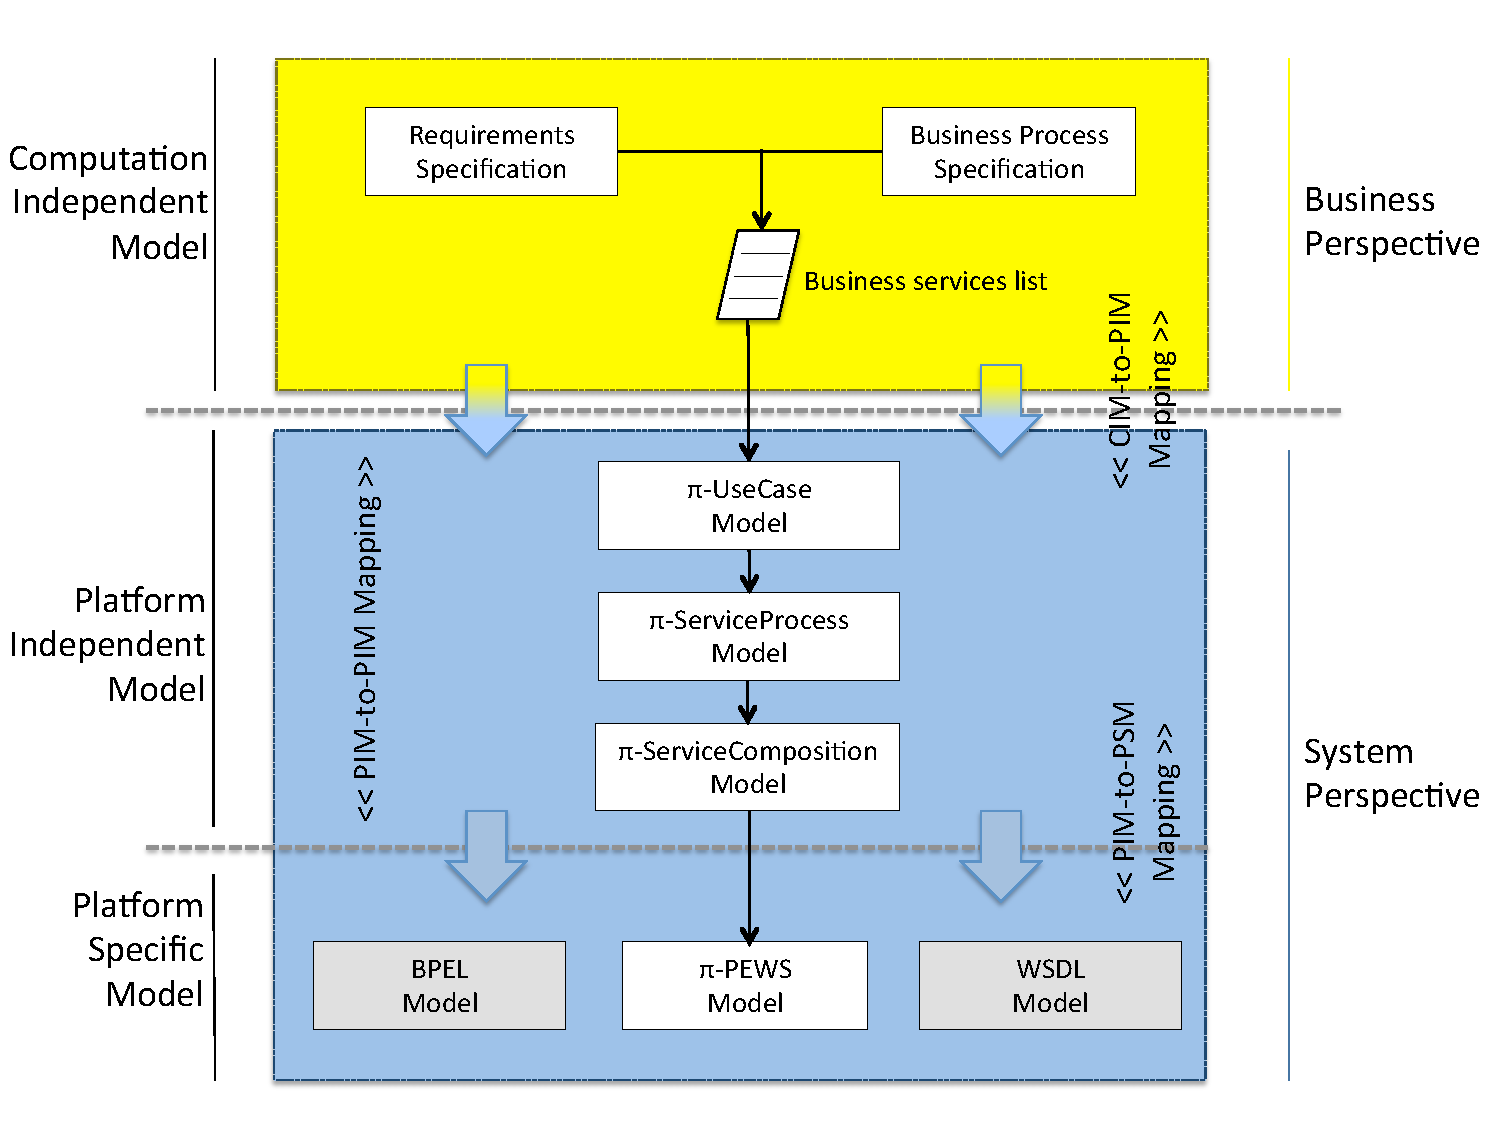
\includegraphics[width=0.5\textwidth]{fig/PiSOD-MProcess}
\caption{$\pi$SOD-M Development Process and Models.}
\label{fig:developmentProcess}
\end{figure}


 Computation Independent Models (CIM) aim to represent the business view, while
 Platform Independent Models (PIM) and Platform Specific Models (PSM) aim
 to represent the information system view and detail the information system to
 be implemented to fulfill the requirements of a business environment.

 Figure \ref{fig:developmentProcess} presents the $\pi$SOD-M development
 process, which defines a service oriented approach providing the guidelines for
 building service-based information systems (SIS), that was the result of the
 SOD-M extension described in figure \ref{fig:sodmExtensions}. 
 
\subsection{Running Example}


In order to introduce the context of our research, consider a \textit{tracking
crime} application where civil population and by police share information about
criminality in given zones of an imaginary city, where: 

\begin{enumerate}
  \item users signal crimes using twitter and police officers notify crimes 
  they have to deal with; 
  \item some of this information if it is not confidential can be shared to the
  community of users using this application;
  \item users can track crimes in given zones and see information located in a
  map according to their privileges: 
  \begin{enumerate}
    \item civilians can ask to \textit{locate the crimes done the last month 100 km
    from my current position that happened between 8:00 and 14:00}; 
    \item police officers can ask to \textit{locate the regions in my sector where
    murders happened in the last month}.
  \end{enumerate}
   \item informations can come from the police database and from twitter
   posts; 
  \item the zones of the city are defined thereby according to their degree of
  criminality.

\end{enumerate}

 In order to provide these functions the application benefits from existing
 services that provide information, that provide storage and data visualization
 functions. Thus, the application is a service based application that implements
 a business process described as figure \ref{fig:example}. 
 \begin{figure}[ht!]
\centering

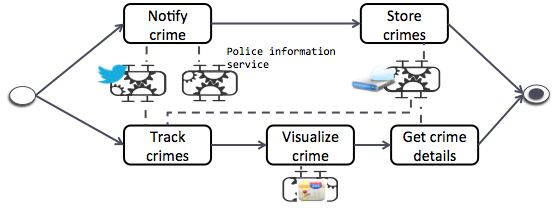
\includegraphics[width=.5\textwidth]{fig/businessProcess.png}

\caption{Business Process Definition Example.}
\label{fig:example}
\end{figure}
 
 
\section{WS-BPEL Processes Generation}

\subsection{Model to Model Transformation}

\subsection{Model to Text Transformation}

\section{Experiments and Results}


\section{Final Remarks}
The conclusion goes here.




% conference papers do not normally have an appendix


% use section* for acknowledgement
% \section*{Acknowledgment}
% 
% 
% The authors would like to thank... 





% trigger a \newpage just before the given reference
% number - used to balance the columns on the last page
% adjust value as needed - may need to be readjusted if
% the document is modified later
%\IEEEtriggeratref{8}
% The "triggered" command can be changed if desired:
%\IEEEtriggercmd{\enlargethispage{-5in}}

% references section

% can use a bibliography generated by BibTeX as a .bbl file
% BibTeX documentation can be easily obtained at:
% http://www.ctan.org/tex-archive/biblio/bibtex/contrib/doc/
% The IEEEtran BibTeX style support page is at:
% http://www.michaelshell.org/tex/ieeetran/bibtex/
%\bibliographystyle{IEEEtran}
% argument is your BibTeX string definitions and bibliography database(s)
%\bibliography{IEEEabrv,../bib/paper}
%
% <OR> manually copy in the resultant .bbl file
% set second argument of \begin to the number of references
% (used to reserve space for the reference number labels box)


\bibliography{biblio}
\bibliographystyle{plain}
 
% \begin{thebibliography}{1}
% 
% \bibitem{IEEEhowto:kopka}
% H.~Kopka and P.~W. Daly, \emph{A Guide to \LaTeX}, 3rd~ed.\hskip 1em plus
%   0.5em minus 0.4em\relax Harlow, England: Addison-Wesley, 1999.
% 
% \end{thebibliography}




% that's all folks
\end{document}


 